%!TEX root = ../../../thesis.tex

Details of components in the electrode-electrolyte interface model and methods of determining its parameters have been discussed.
The focus now moves to measuring and fitting of the model parameters to the model.
Model parameters will first be determined for various concentrations of phosphate buffered saline (PBS), and then for comparison -- in a living sheep's spinal cavity.
This tells us whether a one-tenth concentration of PBS is in-fact a good substitute for cerebrospinal fluid (CSF), which it is assumed to be by implant engineers.

\section{Phosphate Buffered Saline}
    Scott \& Single fitted parameters of their model to a one-tenth concentration (0.1X) of a standard solution of PBS \cite{Scott2014}.
    I measure and fit parameters not only to the one-tenth concentration of PBS but to a range of concentrations from 0.025X up to 1X.
    Not all of the model parameters vary with concentration, but for the ones that do, a fit of the parameter's value to concentration using regression analysis has been made. %TODO: Correct punctuation in this sentence?%
    Doing this gives a a model that can be used to predict the impedance response of an electrode array in a wide range of solution concentrations.

    Each of the PBS measurements were made in \SI{1}{\litre} glass bottles containing \SI{700}{\milli\litre} of PBS solution in each case.
    Measurements were made in a controlled environment maintaining an ambient temperature of \SI{23}{\degree} Celsius.
    All measurements were automated by the use of Python scripts running on a GNU/Linux based workstation.
    The scripts communicate with the instruments both to configure measurements and collect data.
    Each measurement set was repeated for each of the six concentrations of PBS used.
    % The six concentrations of PBS measured are 0.025X, 0.05X, 0.1X, 0.25X 0.5X, and 1.0X the concentration of the standard stock solution.
    The six concentration of PBS measured are shown in \cref{tab:pt2-PBS_concentrations}.
    \begin{table}
      \centering
      \begin{tabular}{l}
        Concentration\\
        \hline
        1.00X\\
        0.5X\\
        0.25X\\
        0.1X\\
        0.05X\\
        0.025X\\
      \end{tabular}
      \caption{\label{tab:pt2-PBS_concentrations}Six PBS concentrations used to fit model parameters to.}
    \end{table}

    \subsection{Resistor Mesh}

      \begin{figure}
        \centering
        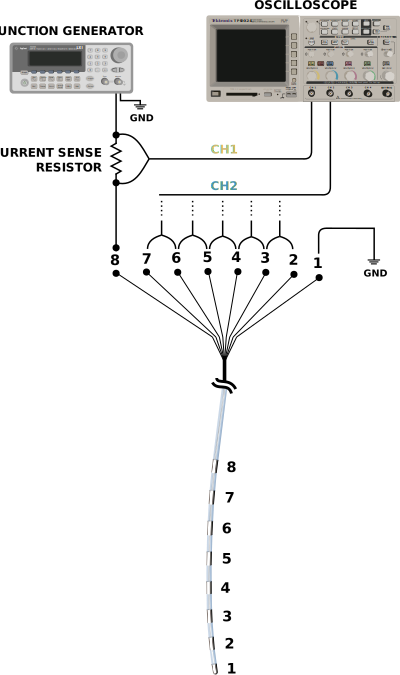
\includegraphics{content/pt2/08-InterfaceParameters/graphics/measurement_resistorMesh}
        \caption{\label{fig:pt2-measurement_resistorMesh}Illustration of one of two measurement configurations used to to measure the electrode transimpedances. Each of the electrode pairs were measured one-after-the-other using the shown equipment.}
      \end{figure}

      With the electrode immersed in a solution of PBS a \SI{10}{\kilo\hertz} sinusoidal current having an amplitude of \SI{500}{\micro\ampere} was passed through the stimulus electrodes using an Agilent 33220A function generator.
      A current sense resistor was inserted in series with the stimulus electrodes.
      The differential voltage across a pair of non-stimulating electrodes and the voltage across the current sense resistor was measured using a Tektronix TPS 2024 oscilloscope.
      \Cref{fig:pt2-measurement_resistorMesh} shows the measurement configuration used when electrodes one and eight are used as the stimulus electrodes.
      The second configuration has electrodes 8 and 7 as stimulus electrodes and the remaining electrode pairs are used to measure transimpedance voltage differentials.

      \begin{figure}
        \centering
        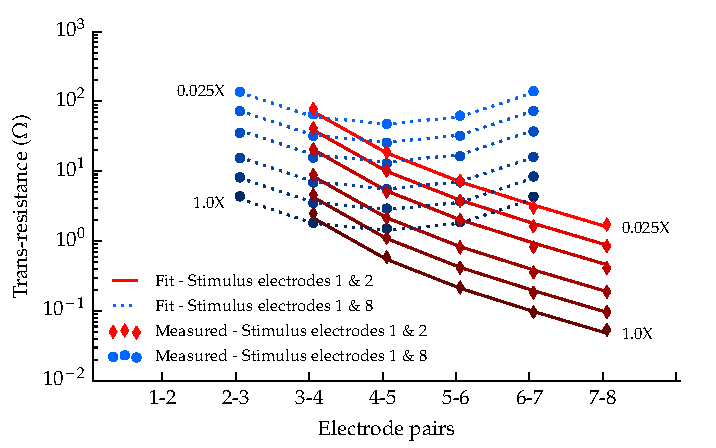
\includegraphics{content/pt2/07-InterfaceModel/graphics/graph_transimpedance_pbs}
        \caption{\label{fig:pt2-graph_transimpedance_pbs}Measured and fitted values of trans-impedance for both measurement configurations. Voltage measurements are made between adjacent pairs of electrodes as current is pushed through the stimulus electrodes.}
      \end{figure}
      The results of those measurements, in both configurations, are shown by markers in \cref{fig:pt2-graph_transimpedance_pbs}.
      Each point is calculated by taking the voltage differential across a pair of electrodes ($V_{diff}$) and dividing by the stimulus current of \SI{500}{\micro\ampere}.
      \begin{table}
        \centering
        \begin{tabular}{r | l}
          Parameter & Value \\
          \hline
          $R_{eri}$ ($\Omega$)& 0.407 / $\sigma$\\
          $R_{sri}$ ($\Omega$)& $R_{eri}\cdot 3/4$\\
          $R_{li}$ ($\Omega$)& 3.71 / $\sigma$ \\
          Depth (layers) & 5 \\
          Padding (layers) & 3 \\
        \end{tabular}
        \caption{\label{tab:RESparams}Resistor mesh parameters. Electrolyte conductivity ($\sigma$) is expressed in units of $S / cm$.}
      \end{table}

      Values for $R_{eri}$ and $R_{li}$ are using a custom Python optimisation script employing the NumPy library for each concentration of PBS.
      The optimisation script selects candidate values for $R_{eri}$ and $R_{li}$, simulates the mesh using those values, and then calculates the equivalent trans-impedance values.
      The error between simulated trans-impedance values and measured values is calculated and the process repeats, selecting different values of $R_{eri}$ and $R_{li}$ to improve the fit.
      The final values of $R_{eri}$ and $R_{li}$ are those that minimise the error, they are shown in \cref{tab:RESparams}.
      $R_{sri}$ is a dependent variable, so is expressed in terms of $R_{eri}$, and the remaining parameters have been re-used from the work of Scott \& Single.
      \Cref{fig:pt2-graph_transimpedance_pbs} shows measurement results for each pair of non-stimulated pair of electrodes along with simulated results using the fitted parameters.


    \subsection{Series Resistance And Constant Phase Element}
      \begin{figure}
        \centering
        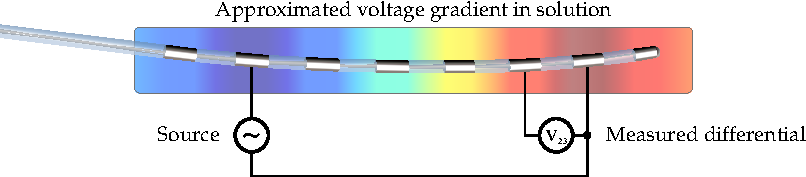
\includegraphics{content/pt2/08-InterfaceParameters/graphics/measurement_CPE}
        \caption{\label{fig:pt2-measurement_CPE}Illustrated voltage gradient in electrolyte solution at each electrode's surface when potential is applied across electrodes two and seven. Measurement of electrolyte voltage taken between electrodes 2 and 3.}
      \end{figure}
      Measurement of both the CPE and the interface's series resistance is made using impedance spectroscopy methods.
      A sinusoidal current is passed between electrodes two and seven of the electrode array.
      Use of the end electrodes (one and eight) was avoided as a precaution to reduce end effects.
      The sinusoidal voltage at the liquid side of the interface is taken as the the voltage that appears at an adjacent electrode (electode three) when a suitably high impedance measurement is made, this is illustrated in \cref{fig:pt2-measurement_CPE}.
      This measurement relies on the ability to make high impedance voltage measurements to minimise voltage drop across the electrode interface, for which a Tektronix TPS 2024 four channel oscilloscope was used.
      All four of its channels are floating and have an input resistance of \SI{10}{\mega\ohm} using 10X probes.
      An Agilent 33220A Function Generator was used to generate the stimulus waveforms applied between electrodes two and eight.
      A series resistance of \SI{10}{\kilo\ohm} was inserted in series with the waveform generator's output.
      It serves as a current sense resistor, also measured using the oscilloscope.
      \begin{figure}
          \centering
          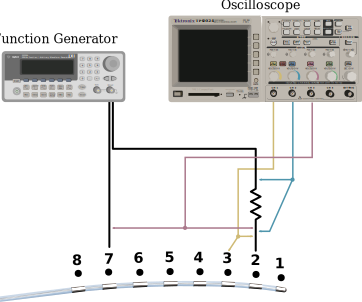
\includegraphics[scale=0.95]{content/pt2/08-InterfaceParameters/graphics/measurement_CPE_setup}
          \caption{\label{fig:pt2-measurement_CPE_setup}Diagram showing the measurement configuration used to measure the CPE response and interface series resistance.}
      \end{figure}
      By measuring the current through electrode two and the voltage across electrodes two's interface, the impedance of the interface can be calculated.
      A diagram showing the measurement setup is shown as \cref{fig:pt2-measurement_CPE_setup}.
      For each of the six solutions, twenty frequencies (log-spaced) were sampled between \SI{50}{\milli\hertz} and \SI{10}{\kilo\hertz} for the impedance measurements.
      At each frequency the stimulus waveform amplitude was re-adjusted to be \SI{300}{\milli\volt}-peak as the interface's impedance changed.
      \begin{figure}
        \centering
        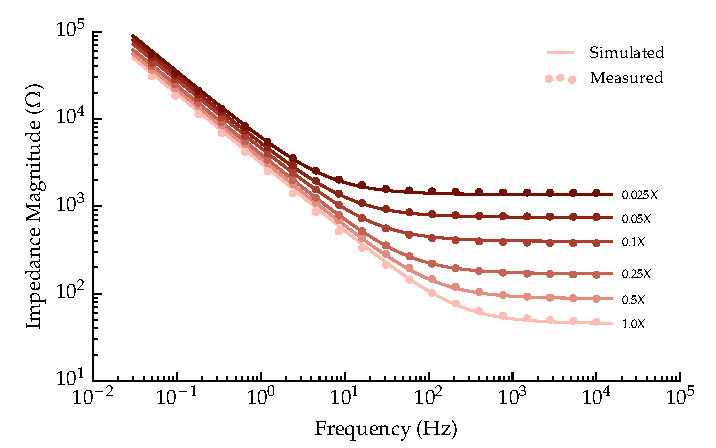
\includegraphics{content/pt2/08-InterfaceParameters/graphics/displacement_impedanceVsFrequency_magnitude_thesis}
        \caption{\label{fig:pt2-graph_impedanceVsFrequency_magnitude}Impedance magnitude of both the measured interface response and the fitted response at each of the six concentrations of PBS.}
      \end{figure}
      \begin{figure}
        \centering
        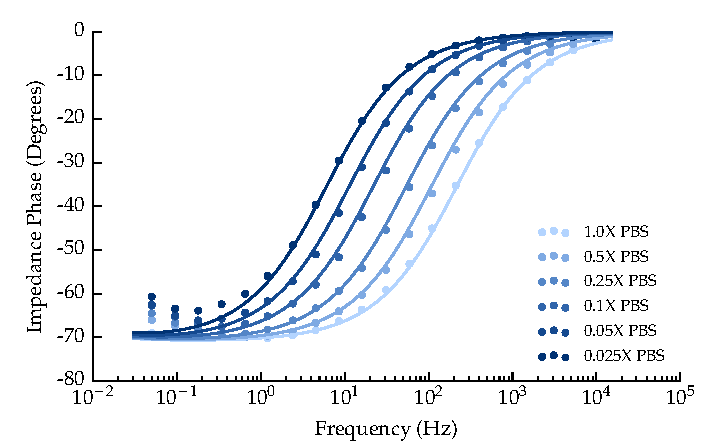
\includegraphics{content/pt2/08-InterfaceParameters/graphics/displacement_impedanceVsFrequency_phase_thesis}
        \caption{\label{fig:pt2-graph_impedanceVsFrequency_phase}Impedance phase of both the measured interface response and the fitted response at each of the six concentrations of PBS.}
      \end{figure}
      \Cref{fig:pt2-graph_impedanceVsFrequency_magnitude,fig:pt2-graph_impedanceVsFrequency_phase} show the calculated impedance magnitude and phase from measurements as markers and simulation results of the fitted parameters as traces.
      \begin{figure}
        \centering
        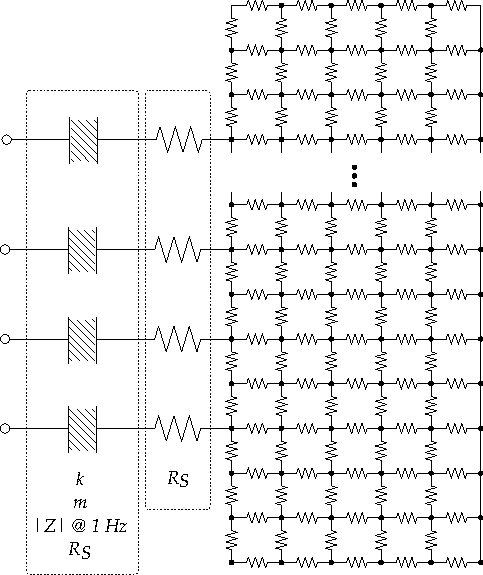
\includegraphics{content/pt2/08-InterfaceParameters/graphics/SpiceModel_opitimisation}
        \caption{\label{fig:pt2-spiceModel_optimisation}The SPICE model schematic used to find optimum values for parameters of the CPE and interface series resistance. Parameters for the resistor mesh are those determined previously.}
      \end{figure}
      \Cref{fig:pt2-spiceModel_optimisation} shows the SPICE model used to simulate parameter values for the CPE and $R_{s}$.
      Final values were found by minimising the difference between the simulated response and the measured response using a Python script.
      For each set of parameter values in the optimisation the script builds a SPICE circuit using those parameter values, simulates the circuit, calculates the interface impedance and compares the values to the measured results.
      The process is automated and runs until a minimum error between simulated and measured results is found.
      Once found, the script exists and displays the final values of each parameter.
      After parameter values are found for each concentration of PBS, another optimisation is made to scale relevant parameters by the concentration.
      The parameters that are scaled with concentration are the series resistance ($R_{S}$) and the CPE's impedance magnitude at \SI{50}{\milli\hertz}.
      The final fit expresses these parameters as functions dependent on the concentration of PBS.
      \begin{figure}
        \centering
        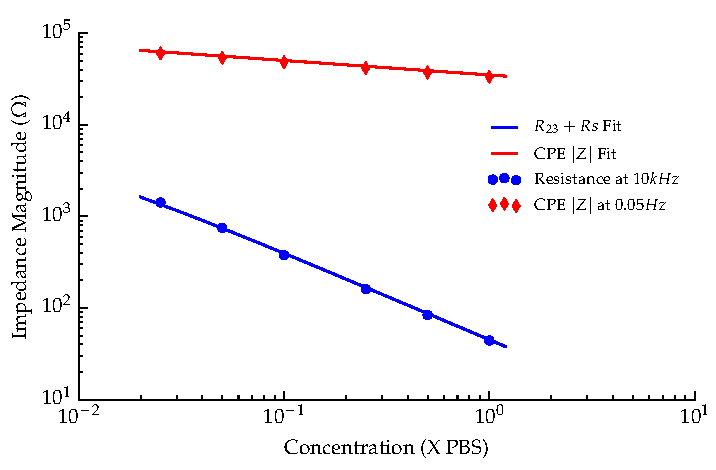
\includegraphics{content/pt2/08-InterfaceParameters/graphics/scalingFactors_Displacement_Thesis}
        \caption{\label{fig:pt2-scalingFactors_Displacement_Thesis}Plot showing fitted parameter values for the CPE impedance magnitude at \SI{50}{\milli\hertz} and series resistance at each of the six concentrations of PBS (shown as markers). The solid trace shows the resulting fit between those values as a function of concentration.}
      \end{figure}
      Individual parameter values for each concentration, along with the resulting fit, is shown in \cref{fig:pt2-scalingFactors_Displacement_Thesis}.
      Measurements of the CPE's vertical position were made at \SI{50}{\milli\hertz}, as opposed to the parameters defined value at \SI{1}{\hertz}, to avoid any effect from the series resistance interfering with the measured value.
      As the slope of the CPE is always the same, the value can be easily converted back to the equivalent value at \SI{1}{\hertz}.
      Measured resistance at high frequency includes the inter-electrode resistance ($R_{23}$) which has been included in the plot, but will be subtracted to leave only $R_{S}$.
      \begin{table}
        \centering
        \begin{tabular}{r | l}
          Parameter & Value \\
          \hline
          $m$& 1.34\\
          $k$ & 1.773\\
          |Z| @ \SI{1}{\hertz} ($\Omega$)& $3284 \times concentration^{-0.158}$ \\
          $R_{S}$ ($\Omega$)& $13.38 \times concentration^{-0.8397}$
        \end{tabular}
        \caption{\label{tab:CPEparams}CPE and $R_{s}$ parameters. Concentration is relative to the stock solution of phosphate buffered saline.}
      \end{table}
      The final parameters for the CPE and $R_{S}$ are given in \cref{tab:CPEparams}.

    \subsection{Faradaic Current}
    \begin{figure}
      \centering
      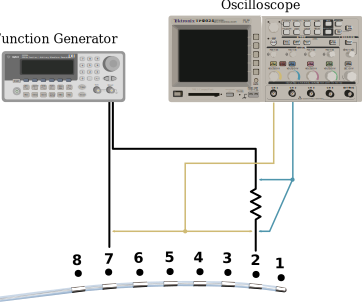
\includegraphics{content/pt2/08-InterfaceParameters/graphics/measurement_Faradaic_setup_initial}
      \caption{\label{fig:pt2-measurement_Faradaic_setup_initial}Illustration of the cyclic voltammetry measurement configuration.}
    \end{figure}
      Using the same oscilloscope and function generator as the previous measurement, the oscilloscope now measures only the voltage between the two electrodes and the current through the current sense resistor.
      The function generator is set to produce a triangle wave, or linear ramp, stimulus between electrodes two and seven.
      Faradaic currents become evident as the electrical current begins to increase exponentially while the voltage moves linearly.
      The point at which the electrical current draw begins to move exponentially with voltage is the point at which the Faradaic reaction begins.



    \subsection{Final Model}

\section{Biological parameter measurements}
    \label{sect:sheep_measurements}
    \subsection{Resistor Mesh}
    \subsection{Series Resistance And Constant Phase Element}
    \subsection{Faradaic Current}
    \subsection{Final Model}
